\section{Auswertung}
Als erstes soll einen Gaußkurve an den Detektor-Scan gefittet werden.
Hierfür wird die Parametrisierung
\begin{equation*}
    f(\theta) = A\exp\left( - \frac{( \theta - \mu)^2}{2\sigma^2} \right)
\end{equation*} 
benutzt, wobei $A$ die Amplitude, $\mu$ der Mittelwert und $\sigma$ die Standardabweichung ist.
Die Halbwertsbreite $\text{FWHM} = 2\sqrt{2\log2}\sigma$ lässt sich aus $\sigma$ berechnen.
Die berechneten Werte sind gegeben durch
\begin{align*}
    \mu &= \SI{7.5(6)e-3}{\degree}, \\
    A &= \num{9.4(1)e5}, \\
    \sigma &= \SI{4.47(6)e-2}{\degree} \\
    \text{FWHM} &= \SI{1.053(15)e-1}{\degree}
\end{align*}
In Abbildung \ref{fig:Detektor} sind die Messwerte des Detektor-Scans und die gefittete Kurve abgebildet.
\begin{figure}
    \centering
    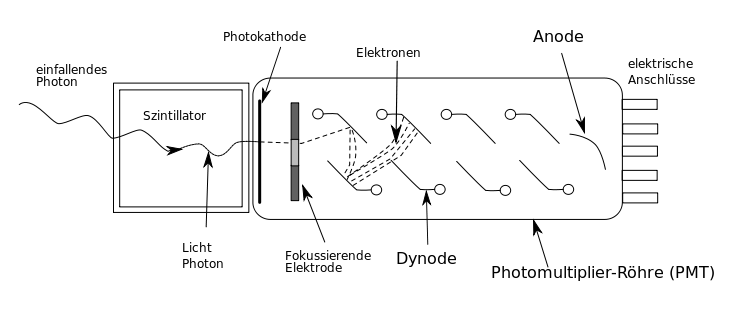
\includegraphics{plots/detektor.pdf}
    \caption{Abbildung des aufgenommen Detektorscanes und den dazu angefertigten Fit. Aufgetragen ist die Intensität gegen den Winkel $\theta$.}
    \label{fig:Detektor}
\end{figure}
Im nächsten Schritt soll der diffusen Scan von dem gemessenen Reflektivitätsscan abgezogen werden. Die Messwerte des Reflektivitätsscans, des diffusen Scans und die Differenz sind in Abbildung \ref{fig:reflekt} abgebildet.
\begin{figure}
    \centering 
    \includegraphics{plots/refklekt.pdf}
    \caption{Der Reflektivitätsscans, der diffuse Scan und die Differenz von beiden. Aufgetragen ist jeweils die Intensität gegen den Winkel $\theta $ in $\si{\degree}$. }
    \label{fig:reflekt}
\end{figure}
In Abbildung \ref{fig:silicium} sind nochmal die Differenz und die Fresnelreflektivität einer ideal glatten Siliziumoberfläche( $n = 1- \num{7.6e-6} + i\num{1.73e-7} $\cite{kiessig}) multipliziert mit der Amplitude $A$ abgebildet.
\begin{figure}
    \centering 
    \includegraphics{plots/ideal.pdf}
    \caption{Die Differenz des Reflektivitätsscans und des diffusen Scans und der Vergleich mit einer Idealen Siliziumoberfläche( $n = 1- \num{7.6e-6} + i\num{1.73e-9} $). Hierbei fällt besonders auf, dass bei der Siliziumoberfläche keine Kiessig-Oszillationen  auftreten, da es sich um ein Einschichtsystem handelt.   }
    \label{fig:silicium}
\end{figure}
Nun soll der Geometriefaktor bestimmt werden um die Daten damit zu anzupassen.
\begin{figure}
    \centering 
    \includegraphics{plots/rocking.pdf}
    \caption{Der Rocking-Scan welcher für die Justage durchgeführt wurde. Aufgetragen ist die Intensität als funktion des Winkel $\theta$, wobei der Winkel zwischen der Röhre und dem Detektor konstant ist. Die rot gepunkteten Linien sind die Schnittpunkte des Graphen mit der Nulllinie. Mit dessen hilfe kann der Geometriewinkel $\theta_g$ bestimmt werden.}
    \label{fig:Dreieck}
\end{figure}
Hierfür wird die Strahlenbreite benötigt, welche aus dem z-Scan \ref{fig:zScan}, zu $d_0 = \SI{0.24}{\milli\meter}$ abgelesen werden kann.
\begin{figure}
    \centering 
    \includegraphics{plots/z_scan.pdf}
    \caption{Der Z-scan, welcher Teil der Justage ist. Aufgetragen ist die Intensität gegen die vertikale Höhe der Probe. Die roten gepunkteten Linien erlauben das ablesen der Strahlenbreite. }
    \label{fig:zScan}
\end{figure}
Bei bekanntem Geometriewinkel $\theta_g$, Strahlenbreite $d_0$ und Probengröße $D$, kann der Geometriefaktor \ref{eq:geometrie} auf zwei verschiedenen Wegen berechnet werden.
Der Geometriewinkel $\theta_g$ kann aus dem Rocking-Scan \ref{fig:Dreieck} abgelesen werden. Hierbei handelt es sich um denn Abstand zwischen dem Nullpunkt und den Enden des Dreieckes und er beträgt $\theta_g = \SI{0.7}{\degree}$.
Die Probengröße wurde vom Praktikumsbetreuer angegeben und beträgt $D = \SI{22}{\mm} $.
Hieraus lässt sich der Wert $\theta_c = \arcsin\left(\frac{d_0}{D}  \right) =\SI{0.63}{\degree} $ berechnen.
Im folgenden sind alle Messdaten mit $\theta < \theta_g$ durch den Faktor $G = \frac{\sin\theta }{\sin\theta_g}$ geteilt.
Die Schichtdicke der Probe lässt sich aus dem modifizierten Reflektivitätsscan \ref{fig:reflekt_norm} bestimmen. Hierfür wurden alle minima $\theta_i$ im Bereich $(0.4,1.0)$, bei welchem die Kiessig-Oszillationen  gut erkennbar sind, abgelesen.
Anschließend können aus den differenzen $\Delta \theta_i = \theta_i - \theta_{i-1}$ die Schichtdicken bestimmt werden. Die abgelesenen Minima und die daraus berechneten Wellenvektorüberträge und Schichtdicken sind in Tabelle \ref{tab:minima} eingetragen.
\begin{figure}
    \centering
   % \begin{subfigure}[]{0.48\textwidth}
   %     \includegraphics{plots/refklekt_norm.pdf}
   % \end{subfigure}
    %\begin{subfigure}[]{0.48\textwidth}
        \includegraphics{plots/refklekt_norm_zoom.pdf}
    %\end{subfigure}
    \caption{Der Reflektivitätsscan modifiziert mit dem Geometriefaktor, wie im Text beschrieben. Aufgetragen ist die Intensität gegen den Winkel $\theta$. Hier ist der Winkelbereich $(0.4°,1.0°)$ gezeigt, um das Ablesen der $11$ Minima für Tabelle \ref{tab:minima} zu ermöglichen.  }
    \label{fig:reflekt_norm}
\end{figure}
\begin{table}
    \centering
    \begin{tabular}{@{}llll@{}}
    \toprule
     $\theta_i/ \si{\degree}$&$\Delta \theta_i / \si{\degree}$&$\Delta q / \SI{e8}{\per\metre} $&$d / \si{\nano\metre} $  \\ \midrule
     \num{0.44} &   $– $           &$– $   & $– $  \\
     \num{0.49} &\num{0.05 }   &\num{7.12}       & \num{88.2}  \\
     \num{0.54} &\num{0.05  }   &\num{7.12}      & \num{88.2} \\
     \num{0.59} &\num{0.05  }   &\num{7.12}      & \num{88.2} \\
     \num{0.64} &\num{0.05  }   &\num{7.12}      & \num{88.2} \\
     \num{0.70} &\num{0.06  }   &\num{8.54}      & \num{73.5} \\
     \num{0.75} &\num{0.05  }   &\num{7.12}      & \num{88.2} \\
     \num{0.80} &\num{0.05  }   &\num{7.12}      & \num{88.2} \\
     \num{0.85} &\num{0.05  }   &\num{7.12}      & \num{88.2} \\
     \num{0.91} &\num{0.06  }   &\num{8.54}      & \num{73.5} \\
     \num{0.96} &\num{0.05  }   &\num{7.12}      & \num{88.2} \\ \midrule
      Mittelwerte    &\num{0.051(4)} &\num{7.4(6)}  & \num{85(6)} \\ \bottomrule
    \end{tabular}
    \caption{Werte für die Minima abgelesen auf Abbildung \ref{fig:reflekt_norm} und die berechneten Winkeldifferenzen $\Delta \theta$, Wellenvektorüberträge $\Delta q$ und die Schichtdicken $d$. In der letzten Zeile sind die Mittelwerte und Standardabweichungen, welche aus den $10$ Messwerten berechnet wurden, eingetragen.}
    \label{tab:minima}
\end{table} 
Um das Dispersionsprofil der Probe zu bestimmen, wird der sogenannte Parrat-Algorithmus benutzt, wobei auch die Rauigkeit der Oberfläche berücksichtigt wird. 
Dies ermöglicht die Durchführung eines Fittes der freien Parameter $n_i = 1 -\delta_i +i\beta_i $, die Schichtdicke $z$ und die Rauigkeit $\sigma_i$, wobei $i = 1,2$ für die verschiedenen Schichten( PS und Si) steht. 
Ein allgemeiner Fit an die $5$ Parameter war nicht möglich, weshalb Parameterbereiche und Startwerte als zusätzliche Annahme eingeführt wurden. Diese basieren auf den Werten von der Anleitung \cite{kiessig}. Für den Fit wurde die \texttt{curve\_fit}-Funktion aus \texttt{Scipy} \cite{scipy} benutzt. 
Des weiteren waren die Unsicherheiten auf die Rauigkeiten $\sigma_i$ sehr groß, weshalb ein weiterer Fit durchgeführt wurde, bei welchem $\sigma_1 = \sigma_2$ angenommen wurde. Zuletzt wurde noch ein Fit durchgeführt, bei welchem die Rauigkeiten $\sigma_i$ vernachlässigt wurden. 
Die Parameterbereiche, Startwerte und die Ergebnisse der drei verschiedenen Fits sind in Tabelle \ref{tab:fit} aufgelistet. In Abbildung \ref{fig:fit} sind die Messwerte, geteilt durch die Amplitude $A$, und die Fitkurve abgebildet. 
Die berechneten kritischen Winkel $\theta_c$, basierend auf Formel \ref{eqn:krit} für die verschiedenen Substanzen sind in Tabelle \ref{tab:winkel} eingetragen.
\begin{table}
    \centering
    \begin{adjustbox}{width=1\textwidth}
    \begin{tabular}{@{}llllllll@{}}
    \toprule
     &$z/ \si{\nm} $&$\delta_1/ \num{e-6}$&$\delta_2/ \num{e-6}$&$\beta_1 / \num{e-6}$&$\beta_2/ \num{e-6} $& $\sigma_1  / \SI{e-10}{\metre}$ & $\sigma_2 / \SI{e-10}{\metre}$  \\ \midrule
     Fit 1:                       &[\num{0.01};\num{10}] &[\num{0.1};\num{10}] &[\num{0.1};\num{10}] &[\num{0.1};\num{10}] &[\num{0.1};\num{10}] &[\num{0.1};\num{10}] &[\num{0.1};\num{10}] \\ 
     Startwerte                   &\num{90} &1 & 1 &0.1 &0.1 & 3&8\\
     Fitwerte                     &\num{88.2(11)} &\num{2.0(5)} &\num{2.01(6)} &\num{3.04(15)} &\num{3.02(10)} &\num{1(217)} &\num{9(753)} \\
     rel. Fehler [\%]             &13 &25 &4 &5 &3 &21702 &75390 \\ \midrule 
     Fit 2:$\sigma_1 = \sigma_2$  &[\num{0.01};\num{10}] &[\num{0.1};\num{10}] &[\num{0.1};\num{10}] &[\num{0.1};\num{10}] &[\num{0.1};\num{10}] &[\num{0.1};\num{10}] &[\num{0.1};\num{10}] \\ 
     Startwerte                   &\num{90} &1 & 1 &0.1 &0.1 & 3&8\\
     Fitwerte                     &\num{89(14)} &\num{1.83(8)} &\num{1.838(4)}&\num{3.18(3)} &\num{3.176(9)} &\num{5(342)} &\num{5(342)} \\ 
     rel. Fehler [\%]             &\num{15.7} &\num{4.4} &\num{0.2} &\num{0.3} &\num{0.2} &\num{6212} &\num{6212} \\ \midrule
     Fit 3:$\sigma_i = 0$         &[\num{0.01};\num{10}] &[\num{0.1};\num{10}] &[\num{0.1};\num{10}] &[\num{0.1};\num{10}] &[\num{0.1};\num{10}] &– &– \\ 
     Startwerte                   &\num{90} &1 & 1 &0.1 &0.1 & –&–\\
     Fitwerte                     &\num{90(2)} &\num{2.20(3)} &\num{2.2(9)} &\num{3.147(9)} &\num{3.141(5)} &– &– \\ 
     rel. Fehler  [\%]            &\num{22.67} &\num{1.54} &\num{0.04} &\num{0.08} &\num{0.05} &– &– \\ \bottomrule
    \end{tabular}
    \end{adjustbox}
    \caption{Ergebnisse der verschiedenen Fits der Daten an die Theoriekurve, welche mit dem Parrat-Algorithmus berechnet wurde. Die generelle Vorgehensweise und Annahmen der verschiedenen Fits ist im Detail im Fließtext erläutert. Hier zeigt die erste Zeile jeweils die angenommenen Parameterbereiche, die zweite Zeile die Startwerte und die dritte Zeile die gefitteten Werte. Des Weiteren sind auch die relativen Fehler eingetragen um die generelle Sensitivität auf die verschiedenen Parameter darzustellen. }
    \label{tab:fit}
\end{table} 
\begin{figure}
    \includegraphics{plots/parrat.pdf}
    \caption{Erneute Abbildung des Reflektivitätsscans und die Fitkurve erstellt mithilfe des Parrat-Algorithmus, basierend auf dem Allgemeinen Fit 1. Aufgetragen ist die Intensität normiert auf die Amplitude $A$ als Funktion des Winkels $\theta$. }
    \label{fig:fit}
\end{figure}
\begin{table}
    \centering
    \begin{tabular}{@{}lll@{}}
    \toprule
     &$\theta_{c,PS} $&$\theta_{c,Si} $ \\ \midrule
    Fit 1 &\num{0.115(14)} & \num{0.115(2)}   \\
    Fit 2 &\num{0.110(2)} &\num{0.110(1) }    \\
    Fit 3 &\num{0.1202(9)} &\num{0.12030(3)  }   \\ \bottomrule
    \end{tabular}
    \caption{Die berechneten kritischen Winkel $\theta_c$ basierend auf Formel \ref{eqn:krit} und den Werten $\delta_i$ aus Tabelle \ref{tab:fit}. Erneut sind diese für die verschiedenen Fits berechnet worden. Hier steht PS für die Polysterol-Schicht und Si für den Silizium-Wafer.  }
    \label{tab:winkel}
\end{table} 